\documentclass[a4paper]{article}
\usepackage[margin=3.5cm]{geometry}
\usepackage{amsmath}
\usepackage{amssymb}
\usepackage[svgnames]{xcolor}
\usepackage{amsthm}
% \makeatletter
% \def\th@plain{%
%   \thm@notefont{}% same as heading font
%   \itshape % body font
% }
% \def\th@definition{%
%   \thm@notefont{}% same as heading font
%   \normalfont % body font
% }
% \makeatother
\usepackage{dsfont}
\usepackage{graphicx}
\usepackage{caption}
\usepackage{hyperref}
\usepackage{cleveref}
\usepackage{datetime}
\usepackage{outlines}
\usepackage{float}
\usepackage{booktabs}
\usepackage{enumitem}
\usepackage{tabto}
\usepackage{mathtools}
\usepackage{nicematrix}
\usepackage{nccmath}
\usepackage{lipsum}
\usepackage[activate={true,nocompatibility},final,tracking=true,kerning=true,spacing=true,factor=500,stretch=15,shrink=15]{microtype}

\usepackage{apptools}
\AtAppendix{\counterwithin{lemma}{section}}

\addtolength{\skip\footins}{2mm}

\definecolor{fgcolor}{rgb}{0.345, 0.345, 0.345}
\newcommand{\hlnum}[1]{\textcolor[rgb]{0.686,0.059,0.569}{#1}}%
\newcommand{\hlstr}[1]{\textcolor[rgb]{0.192,0.494,0.8}{#1}}%
\newcommand{\hlcom}[1]{\textcolor[rgb]{0.678,0.584,0.686}{\textit{#1}}}%
\newcommand{\hlopt}[1]{\textcolor[rgb]{0,0,0}{#1}}%
\newcommand{\hlstd}[1]{\textcolor[rgb]{0.345,0.345,0.345}{#1}}%
\newcommand{\hlkwa}[1]{\textcolor[rgb]{0.161,0.373,0.58}{\textbf{#1}}}%
\newcommand{\hlkwb}[1]{\textcolor[rgb]{0.69,0.353,0.396}{#1}}%
\newcommand{\hlkwc}[1]{\textcolor[rgb]{0.333,0.667,0.333}{#1}}%
\newcommand{\hlkwd}[1]{\textcolor[rgb]{0.737,0.353,0.396}{\textbf{#1}}}%
\let\hlipl\hlkwb

\usepackage{framed}
\makeatletter
\newenvironment{kframe}{%
 \def\at@end@of@kframe{}%
 \ifinner\ifhmode%
  \def\at@end@of@kframe{\end{minipage}}%
  \begin{minipage}{\columnwidth}%
 \fi\fi%
 \def\FrameCommand##1{\hskip\@totalleftmargin \hskip-\fboxsep
 \colorbox{shadecolor}{##1}\hskip-\fboxsep
     % There is no \\@totalrightmargin, so:
     \hskip-\linewidth \hskip-\@totalleftmargin \hskip\columnwidth}%
 \MakeFramed {\advance\hsize-\width
   \@totalleftmargin\z@ \linewidth\hsize
   \@setminipage}}%
 {\par\unskip\endMakeFramed%
 \at@end@of@kframe}
\makeatother

\definecolor{shadecolor}{rgb}{.97, .97, .97}
\definecolor{messagecolor}{rgb}{0, 0, 0}
\definecolor{warningcolor}{rgb}{1, 0, 1}
\definecolor{errorcolor}{rgb}{1, 0, 0}
\newenvironment{knitrout}{}{} % an empty environment to be redefined in TeX


% code highlighting
\usepackage{minted}
\usepackage{xpatch}
\newminted[cminted]{python}{fontsize=\small}
\xpretocmd{\cminted}{\RecustomVerbatimEnvironment{Verbatim}{BVerbatim}{}}{}{}

% link coloring
\hypersetup{
   colorlinks,
   linkcolor={red!90!black},
   citecolor={green!40!black},
   urlcolor={blue!60!black}
}

% concatenation symbol (c.f. ++ in Haskell)
\newcommand\mdoubleplus{\mathbin{+\mkern-10mu+}}

% end of proof symbol
\newcommand{\newmarkedtheorem}[1]{%
  \newenvironment{#1}
    {\pushQED{\qed}\csname inner@#1\endcsname}
    {\popQED\csname endinner@#1\endcsname}%
  \newtheorem{inner@#1}%
}
% \renewenvironment{proof}{{\noindent\bfseries Proof.}}{*something*}
%\let\oldproofname=\proofname
%\renewcommand{\proofname}{\rm\bf{\oldproofname}}


\theoremstyle{definition}
%\newtheorem{eg}{Example}[section]
\newmarkedtheorem{eg}{Example}[section]
\newtheorem{remark}{Remark}
\theoremstyle{plain}
\newtheorem{define}{Definition\hspace{0.25em}\ignorespaces}
\newtheorem{property}{Property\hspace{0.25em}\ignorespaces}
\newtheorem{observation}{Observation}
\newtheorem{proposition}{Proposition}
\newtheorem{lemma}{Lemma\hspace{0.25em}\ignorespaces}
\newtheorem{corollary}{Corollary}
\newtheorem{theorem}{Theorem\hspace{0.25em}\ignorespaces}
\newtheorem{assump}{Assumption\hspace{0.25em}\ignorespaces}

\DeclareMathOperator{\interior}{int}
\DeclareMathOperator*{\argmax}{arg\,max}
\DeclareMathOperator*{\argmin}{arg\,min}
\newcommand*\diff{\mathop{}\!\mathrm{d}}

% cref settings
\crefname{equation}{equation}{equations}
\newcommand{\crefrangeconjunction}{--}

\newdateformat{monthyeardate}{\monthname[\THEMONTH] \THEYEAR}

\author{Jeroen van Riel}
\date{\monthyeardate\today}

\title{Trajectory optimization for vehicles in a lane model with minimum
  following distance and boundary conditions}

\begin{document}

\maketitle

\begin{abstract}
  This section considers a model of a single-lane road on which overtaking is
  not allowed.
  %
  Vehicles are modeled as double integrators with bounds on speed and
  acceleration. Consecutive vehicles must keep some fixed \textit{following
    distance} to avoid collisions.
  %
  It is assumed that vehicles enter and exit the lane at
  predetermined \textit{schedule times}. Whenever a vehicle enters or exits, it
  must drive at full speed.
  %
  For an optimization objective that, roughly speaking, minimizes the distance
  to the end of the lane at all times, we present an algorithm to compute an
  optimal set of trajectories.
  %
  Assuming some minimum lane length, we characterize feasibility of this
  trajectory optimization problem in terms of a system of linear inequalities
  involving the schedule times.
  %
\end{abstract}

% \tableofcontents

\newcommand\halfopen[2]{\ensuremath{[#1,#2)}}
\newcommand\openhalf[2]{\ensuremath{(#1,#2]}}

\renewcommand{\labelitemii}{\textbullet}
\renewcommand{\labelitemiii}{\textbullet}

\section{Lane model}

Vehicles are modeled as double integrators with bounded speed and acceleration,
which means that we only consider their longitudinal position on the road. Let
$\mathcal{D}[a,b]$ denote the set of valid \emph{trajectories}, which we define to be
all continuously differentiable functions $x : [a,b] \rightarrow \mathbb{R}$ satisfying
the constraints
\begin{align}
  0 \leq \dot{x}(t) \leq 1 \quad \text{ and } \quad
  {-\omega} \leq \ddot{x}(t) \leq \bar{\omega} , \quad \text{ for all } t \in [a,b] ,
\end{align}
for some fixed acceleration bounds $\omega, \bar{\omega} > 0$. Note that we use $\dot{x}$
and $\ddot{x}$ to denote the first and second derivative with respect to time
$t$. When we have a general positive speed upper bound, we can always apply an
appropriate scaling of the time axis and the acceleration bounds to obtain the
form.
%
Consider positions $A, B \in \mathbb{R}$, such that $B \geq A$, which denote the
start\footnote{We could have assumed $A=0$, but we will later piece together
  multiple lanes to model intersections.} and end position of the lane.
%
Let $\bar{D}[a, b] \subset \mathcal{D}[a, b]$ denote the set of trajectories $x$ that
satisfy the boundary conditions
\begin{align}
  x(a) = A \; \text{ and } \; x(b) = B .
\end{align}
Even further, let $D[a,b] \subset \bar{D}[a, b]$ induce the boundary conditions
\begin{align}
  \dot{x}(a) = \dot{x}(b) = 1 .
\end{align}
In words, these boundary conditions require that a vehicle arrives to and
departs from the lane at predetermined times $a$ and $b$ and do so at full
speed.

Let $L > 0$ denote the required \textit{following distance} between consecutive
vehicles.
%
Suppose we have $N$ vehicles that are scheduled to traverse the lane. For each
vehicle $i$, let $a_{i}$ and $b_{i}$ denote the \textit{schedule time} for entry
and exit, respectively. A feasible solution consists of a sequence of
trajectories $x_{1}, \dots, x_{N}$ such that
\begin{subequations}\label{eq:feasibility}
\begin{align}
x_{i} \in D[a_{i}, b_{i}] \quad \quad & \text{ for each } i, \\
x_{i} \leq x_{i-1} - L \quad \quad &\text{ for each } i \geq 2,
\end{align}
\end{subequations}
%
where we use the shorthand notation $\gamma_{1} \leq \gamma_{2}$ to mean
$\gamma_{1}(t) \leq \gamma_{2}(t)$ for all
$t \in [a_{1}, b_{1}] \cap [a_{2}, b_{2}]$, given some
$\gamma_{1} \in \mathcal{D}[a_{1}, b_{1}]$ and
$\gamma_{2} \in \mathcal{D}[a_{2}, b_{2}]$.
% We use $\gamma \leq \min \{ \gamma_{1}, \dots, \gamma_{n} \}$ as a shorthand for $\gamma \leq \gamma_{1}, \dots, \gamma \leq \gamma_{n}$.

As optimization objective, we will consider
\begin{align}\label{eq:objective}
  \max \; \sum_{i=1}^{N} \int_{a_{i}}^{b_{i}} x_{i}(t) \diff t ,
\end{align}
which, roughly speaking, seeks to keep all vehicles as close to the end of the
lane at all times.
%
In particular, we will show that optimal trajectories can be understood as the
concatenation of at most four different types of trajectory parts. Based on this
observation, we present an algorithm to compute optimal trajectories.
%
Assuming $(\omega, \bar{\omega},A,B,L)$ to be fixed, with lane length $B-A$
sufficiently large, we will show that feasibility of the trajectory optimization
problem is completely characterized by a system of linear inequalities in
$a_{i}$ and $b_{i}$.

Note that objective~\eqref{eq:objective} does not capture energy efficiency in
any way. Although this is not desirable in practice, it is precisely this
assumption that enables the analysis in this section. Deriving a similar
characterization of feasibility and optimal trajectories under an objective that
does model energy concumption is an interesting topic for further research.

\section{Single vehicle problem}

We will first consider a somewhat generalized version of the
constraints~\eqref{eq:feasibility} for a single vehicle $i$. Therefore, we
lighten the notation slightly by dropping the vehicle index $i$ and instead of
$x_{i-1} - L$, we assume we are given some arbitrary \emph{lead vehicle
  boundary} $\bar{x} \in \bar{D}[\bar{a}, \bar{b}]$, then we consider the
optimization problem
\begin{align}
  \max_{x \in D[a, b]} \int_{a}^{b} x(t) \diff t \quad \text{ such that } \quad x \leq \bar{x} .
\end{align}
to which we will refer as the \emph{single vehicle problem}.

\subsection{Necessary conditions}

For every trajectory $x \in D[a,b]$, we derive two upper
bounding trajectories $x^{1}$ and $\hat{x}$ and one lower bounding trajectory
$\check{x}$, see Figure~\ref{fig:necessary-conditions}.
%
Using these bounding trajectories, we will then formulate four necessary
conditions for feasibility of the single vehicle problem.

Let the \emph{full speed boundary} $x^{1}$ be defined as
\begin{align}
  x^{1}(t) = A + t - a,
\end{align}
for all $t \in [a, b]$, then we clearly have $x \leq x^{1}$.
%
Next, since deceleration is at most $\omega$, we have
$\dot{x}(t) \geq \dot{x}(a) - \omega(t - a) = 1 - \omega(t - a)$, which we
combine with the speed constraint $\dot{x} \geq 0$ to derive
$\dot{x}(t) \geq \max\{0, 1 - \omega (t - a) \}$. Hence, we obtain the lower
bound
\begin{align}\label{eq:check-x}
  x(t) = x(a) + \int_{a}^{t} \dot{x}(\tau) \diff \tau \geq A + \int_{a}^{t} \max\{0, 1 - \omega (\tau - a) \} \diff \tau =: \check{x}(t) .
\end{align}
%
Analogously, we derive an upper bound from the fact that acceleration is at most $\bar{\omega}$. Observe that we have
$\dot{x}(t) + \bar{\omega} (b - t) \geq \dot{x}(b) = 1$, which we combine
with the speed constraint $\dot{x}(t) \geq 0$ to derive
$\dot{x}(t) \geq \max \{ 0, 1 - \bar{\omega}(b - t) \}$. Hence, we obtain the
upper bound
\begin{align}\label{eq:hat-x}
  x(t) = x(b) - \int_{t}^{b} \dot{x}(\tau) \diff \tau
  \leq B - \int_{t}^{b} \max\{ 0, 1 -\bar{\omega} (b - \tau) \} \diff \tau =: \hat{x}(t) .
\end{align}
%
We refer to $\check{x}$ and $\hat{x}$ as the \emph{entry boundary} and
\emph{exit boundary}, respectively.


\begin{figure}
  \centering
  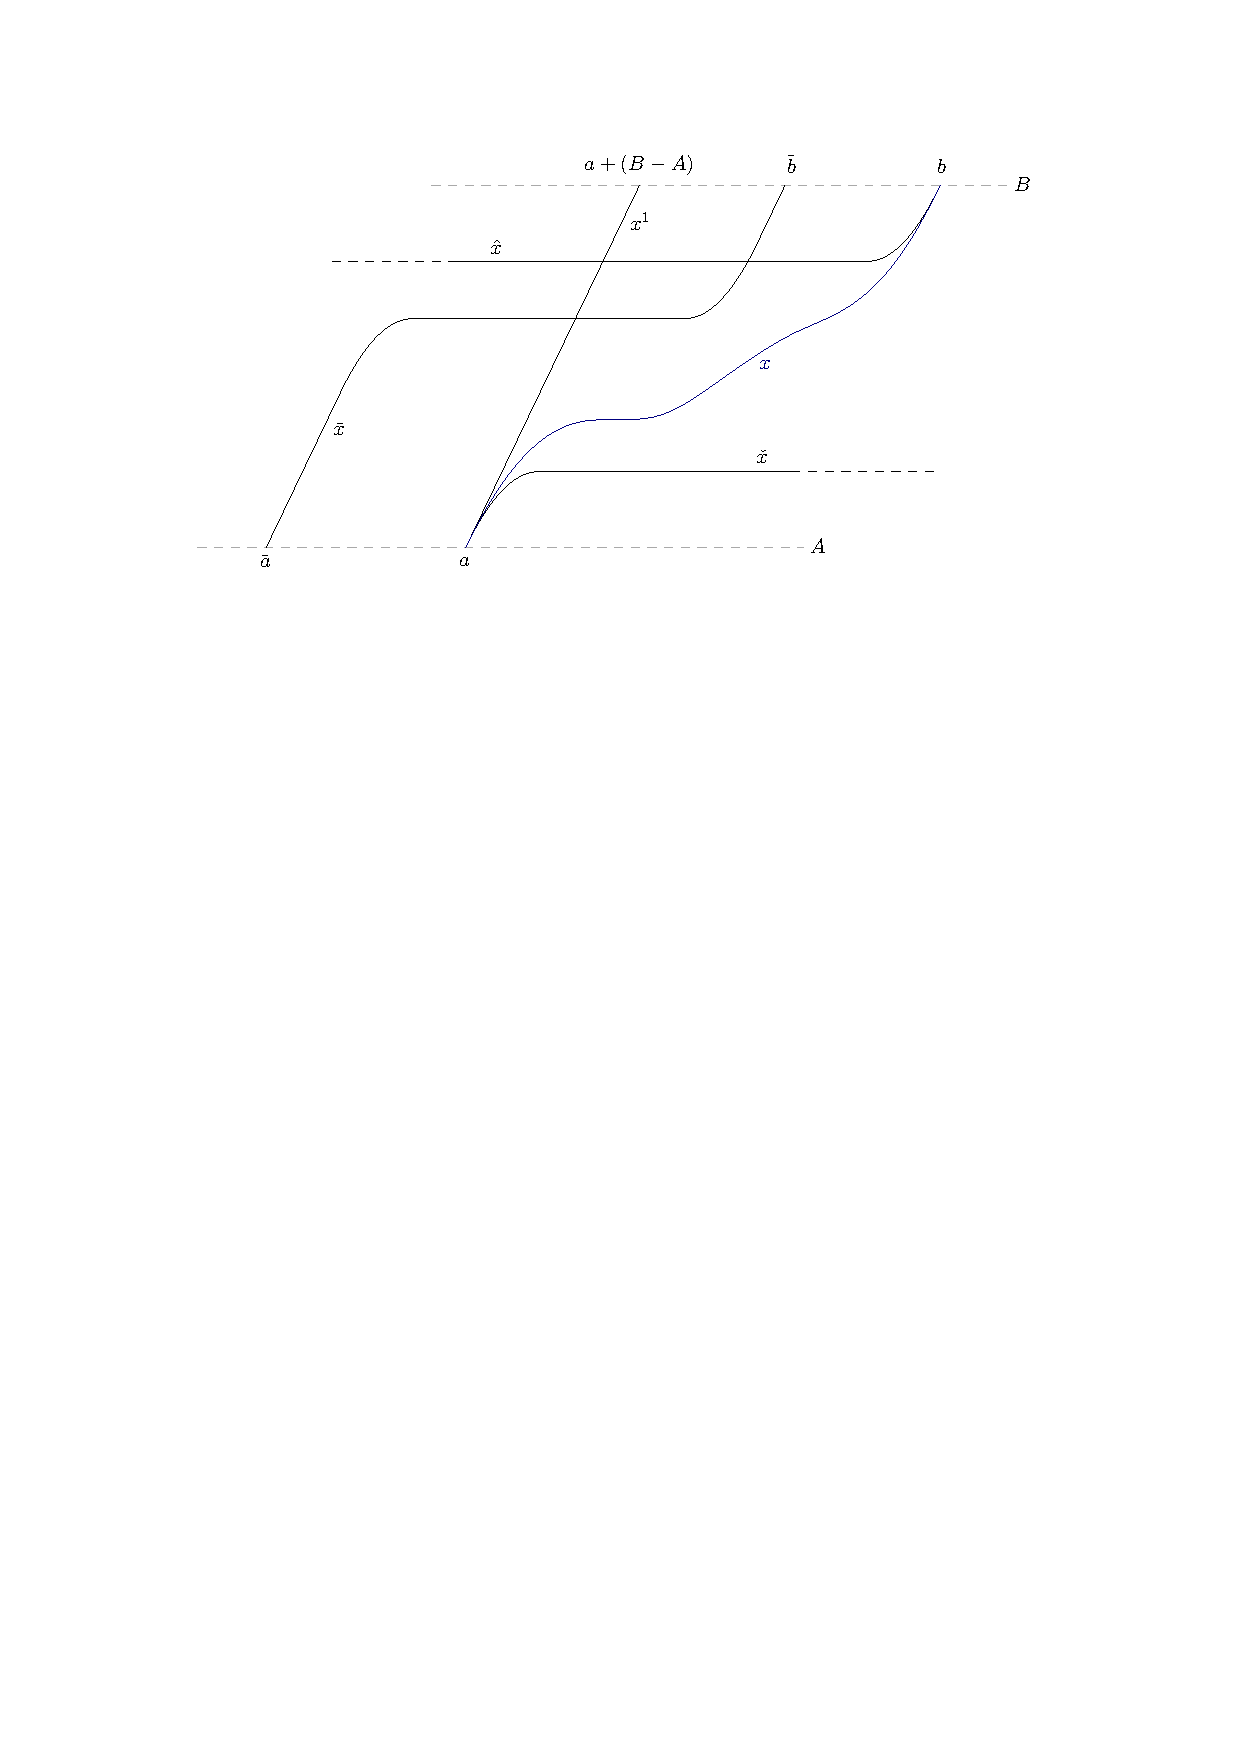
\includegraphics[scale=1]{figures/motion/rough/necessary-conditions}
  \caption{Illustration of the four bounding trajectories
    $\bar{x}, x^{1}, \hat{x}, \check{x}$ that bound feasible trajectories from
    above and below. We also drew an example of a feasible trajectory $x$ in
    blue. The horizontal axis represents time and the vertical axis corresponds
    to the position on the lane, so the vertical dashed grey lines correspond to
    the start and end of the lane.}%
  \label{fig:necessary-conditions}
\end{figure}

\pagebreak

\begin{lemma}\label{lemma:necessary-conditions}
  Let $\bar{x} \in \bar{D}[\bar{a}, \bar{b}]$ and assume there exists a
  trajectory $x \in D[a, b]$ such that $x \leq \bar{x}$, then the following
  conditions must hold \TabPositions{3cm}
  \begin{enumerate}[label=(\roman*)\quad,leftmargin=5em]
    \item $b-a \geq B-A$, \tab (full speed constraint)
    \item $\bar{b} \leq b$, \tab (downstream order constraint)
    \item $\bar{a} \leq a$, \tab (upstream order constraint)
    \item $\bar{x} \geq \check{x}$. \tab (entry space constraint)
  \end{enumerate}
\end{lemma}
\begin{proof}
  Each of the conditions corresponds somehow to one of the four bounding
  trajectories defined above.
  %
  Observe that $x^{1}(t) = B$ for $t = a + (B-A)$, which can be interpreted as
  the earliest time of departure from the lane. This shows that
  $b \geq a + (B-A)$, which is equivalent with (i).
  %
  % When (i) is violated, $x$ must cross $x^{1}$ somewhere, which means that the
  % maximum speed constraint must be violated.
  When either (ii) or (iii) is violated, the constraint $x \leq \bar{x}$
  conflicts with one of the boundary conditions $x(a) = A$ or $x(b) = B$. To see
  that (iv) must hold, suppose that $\bar{x}(\tau) < \check{x}(\tau)$ for some
  time $\tau$. Since $\bar{a} \leq a$, this means that $\bar{a}$ must intersect
  $\check{a}$ from above. Therefore, any trajectory that satisfies
  $x \leq \bar{x}$ must also intersect $\check{a}$ from above, which contradicts
  the assumption that $x$ was a feasible solution.
\end{proof}

We show that the boundaries $\hat{x}$ and $\check{x}$ together could yield yet
another necessary condition. It is straightforward to verify
from~\cref{eq:hat-x,eq:check-x} that $\hat{x}(t) \geq B - 1/(2\bar{\omega})$ and
$\check{x}(t) \leq A + 1/(2\omega)$. Therefore, whenever
$B - A < 1/(2\bar{\omega}) + 1/(2\omega)$, these boundaries intersect for
certain values of $a$ and $b$. Because the exact condition is somewhat
cumbersome to characterize, we avoid this case by simply assuming that the lane
length is sufficiently large.

\begin{assump}\label{eq:AB-assumption}
  The length of the lane satisfies $B - A \geq 1/(2\omega) + 1/(2\bar{\omega})$.
\end{assump}

\pagebreak

\subsection{Constructing the optimal trajectory}

Assuming the four conditions of Lemma~\ref{lemma:necessary-conditions} hold, we will construct an optimal
solution $x^{*}$ for the single vehicle problem, thereby showing that these
conditions are thus also sufficient for feasibility.
%
First, we construct $x^{*}$ by combining the upper boundaries $\bar{x}$,
$\hat{x}$ and $x^{1}$ in a certain way to obtain a smooth trajectory satisfying
$x^{*} \in D[a,b]$.
%
We show that $x^{*}$ is still an upper boundary for any other feasible solution,
which shows that it is optimal.

\begin{figure}
  \centering
  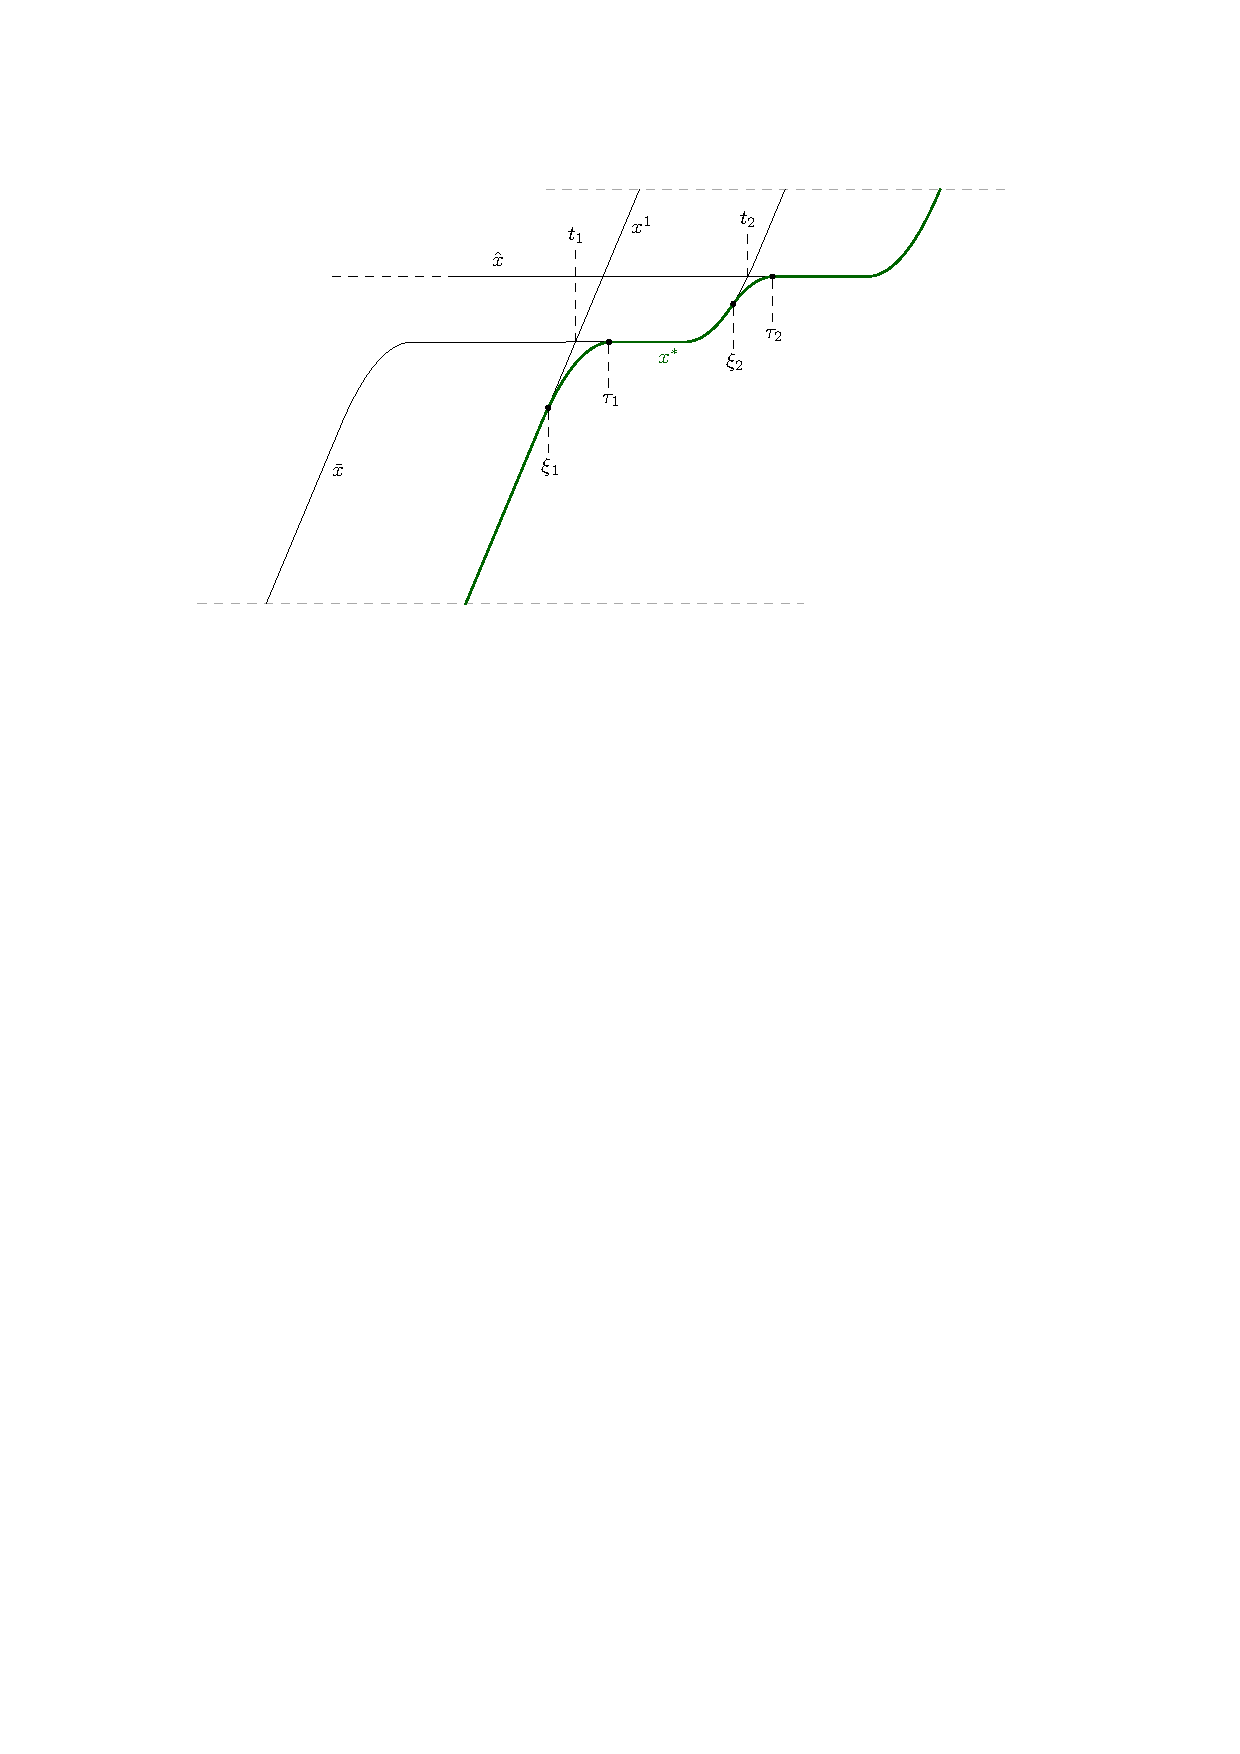
\includegraphics[scale=1]{figures/motion/rough/proof}
  \caption{The minimum boundary $\gamma$, induced by three upper boundaries
    $\bar{x}$, $\hat{x}$ and $x^{1}$, is smoothened around time $t_{1}$ and
    $t_{2}$, where the derivative is discontinuous, to obtain the smooth optimal
    trajectory $x^{*}$, drawn in green. The times $\xi_{i}$ and $\tau_{i}$
    correspond to the start and end of the connecting deceleration boundary as
    defined in Section~\ref{sec:smoothing}.}%
  \label{fig:optimal-construction}
\end{figure}

The starting point of the construction is the \emph{minimum boundary}
$\gamma : [a,b] \rightarrow \mathbb{R}$ induced by the upper boundaries, defined as
\begin{align}\label{eq:min-boundary}
  \gamma(t) := \min \{ \bar{x}(t), \hat{x}(t), x^{1}(t) \} .
\end{align}
%
Obviously, $\gamma$ is still a valid upper boundary for any feasible solution,
%
but in general, $\gamma$ may have a discontinuous derivative at some\footnote{In fact, it can be shown that, under the necessary conditions, there are at most two of such discontinuities.} isolated
points in time.

\begin{define}\label{def:piecewise-trajectory}
  Let $\mathcal{P}[a,b]$ be the set of functions $\mu : [a, b] \rightarrow \mathbb{R}$ for
  which there is a finite subdivision $a = t_{0} < \cdots < t_{n+1} = b$ such that
  the truncation $\mu|_{[t_{i}, t_{i+1}]} \in \mathcal{D}[t_{i}, t_{i+1}]$ is
  a smooth trajectory, for each $i \in \{0, \dots, n\}$, and for which the one-sided limits of $\dot{\mu}$ satisfy
  \begin{align}
    \dot{\mu}(t_{i}^{-}) := \lim_{t \uparrow t_{i}} \dot{\mu}(t) > \lim_{t \downarrow t_{i}} \dot{\mu}(t) =: \dot{\mu}(t_{i}^{+}) ,
  \end{align}
  for each $i \in \{1, \dots, n\}$. We refer to such $\mu$ as a \emph{piecewise
    trajectory (with downward bends)}.
\end{define}

It is not difficult to see from Figure~\ref{fig:necessary-conditions} that,
under the necessary conditions, $\gamma$ satisfies the above definition, so
$\gamma \in \mathcal{P}[a,b]$. In other words, $\gamma$ consists of a number of
pieces that are smooth and satisfy the vehicle dynamics, with possibly some
sharp bend downwards where these pieces come together.
%
Next, we present a simple procedure to smoothen out this kind of discontinuity
by decelerating from the original trajectory somewhat before some $t_{i}$, as
illustrated in Figure~\ref{fig:optimal-construction}. We show that this procedure can be repeated at every
point of discontinuity.

\subsubsection{Deceleration boundary}
In order to formalize the smoothing procedure, we will first define some
parameterized family of functions to model the deceleration part.
%
Recall the derivation of $\check{x}$ in equation~\eqref{eq:check-x} and the discussion
preceding it, which we will now generalize a bit.
%
Let $x \in \mathcal{D}[a, b]$ be some smooth trajectory, then observe that $\dot{x}(t) \geq \dot{x}(\xi) - \omega(t - \xi)$ for all $t \in [a, b]$.
Combining this with the constraint $\dot{x}(t) \in [0, 1]$, this yields
\begin{align}
  \dot{x}(t) \geq \max\{ 0, \, \min\{1, \, \dot{x}(\xi) - \omega (t - \xi) \}\} =: \{\dot{x}(\xi) - \omega(t-\xi)\}_{[0,1]} ,
\end{align}
where use $\{ \cdot \}_{[0,1]}$ as a shorthand for this clipping operation.
%
Hence, for any $t \in [a,b]$, we obtain the following lower bound
\begin{align}\label{eq:stopping-trajectory}
  x(t) = x(\xi) + \int_{\xi}^{t} \dot{x}(\tau) \diff \tau \geq x(\xi) + \int_{\xi}^{t} \{\dot{x}(\xi) - \omega(\tau - \xi)\}_{[0,1]} \diff \tau =: x[\xi] (t) ,
\end{align}
where we will refer to the right-hand side as the \emph{deceleration boundary} of $x$
at $\xi$.
%
Observe that this definition indeed generalizes the definition of $\check{x}$,
because we have $\check{x}=(x[a])|_{[a,b]}$, so $x[a]$ restricted to the
interval $[a,b]$.

Note that $x[\xi]$ depends on $x$ only through the two real numbers $x(\xi)$ and
$\dot{x}(\xi)$. It will be convenient later to rewrite the right-hand side
of~\eqref{eq:stopping-trajectory} as
\begin{align}
  x^{-}[p, v, \xi](t) = p + \int_{\xi}^{t} \{ v - \omega(\tau - \xi) \}_{[0,1]} \diff \tau ,
\end{align}
such that $x[\xi](t) = x^{-}[x(\xi), \dot{x}(\xi), \xi](t)$.
%
We can expand the integral in this expression further by carefully handling
the clipping operation. Observe that the expression within the clipping
operation reaches the bounds $1$ and $0$ for $\delta_{1} := \xi - (1-v)/\omega$ and
$\delta_{0} := \xi + v/\omega$, respectively. Using this notation, a simple calculation
shows that
\begin{align}\label{eq:x-}
  x^{-}[p,v,\xi](t) = p +
  \begin{cases}
    {(1 - v)}^{2} / (2\omega) + (t - \xi) & \text{ for } t \leq \delta_{1} , \\
    v(t - \xi) - \omega{(t-\xi)}^{2} /2 & \text{ for } t \in [\delta_{1} , \delta_{0}] , \\
    v^{2}/(2\omega) & \text{ for } t \geq \delta_{0} .
  \end{cases}
\end{align}
Assuming $0 \leq v \leq 1$, it can be verified that for every $t \in \mathbb{R}$, we
have $\ddot{x}^{-}[p,v,\xi](t) \in \{-\omega, 0\}$ and
$\dot{x}^{-}[p,v,\xi](t) \in [0,1]$ due to the clipping operation, so that
$x^{-}[p,v,\xi] \in \mathcal{D}(-\infty,\infty)$.

\begin{figure}
  \centering
  \includegraphics[scale=1]{figures/motion/rough/stopping-trajectory}
  \caption{Illustration of a deceleration boundary $\mu[\xi]$ of some piecewise
    trajectory $\mu \in \mathcal{P}[a,b]$ at time $\xi$. We truncated $\mu[\xi]$
    for a more compact figure. This particular trajectory $\mu$ has a
    discontinuous derivative at times $t_{1}$ and $t_{2}$. The careful reader
    may notice that this $\mu$ cannot occur as the minimum boundary defined
    in~\eqref{eq:min-boundary}. This only means that the class of piecewise
    trajectories $\mathcal{P}[a,b]$ is just slightly more general than necessary
    for our current purposes.}%
  \label{fig:stopping-trajectory}
\end{figure}

Let $\mu \in \mathcal{P}[a, b]$ be some piecewise trajectory and let
$a = t_{0} < \cdots < t_{n+1} = b$ denote the corresponding subdivision as in
Definition~\ref{def:piecewise-trajectory}, then we generalize the definition of
a deceleration boundary to $\mu$.
%
Whenever $\xi \in [a,b] \setminus \{ t_{1}, \dots, t_{n}\}$, we just define
$\mu[\xi] := x^{-}[\mu(\xi), \dot{\mu}(\xi), \xi]$.
%
However, when $\xi \in \{ t_{1}, \dots, t_{n}\}$, the derivative
$\dot{\mu}(\xi)$ is not defined, so we to use the left-sided limit instead, by
defining $\mu[\xi] := x^{-}[\mu(\xi), \dot{\mu}(\xi^{-}), \xi]$.

Finally, please note that we cannot just replace $x$ with $\mu$ in
inequality~\eqref{eq:stopping-trajectory} to obtain a similar bound for the
whole interval $[a,b]$.
%
Instead, consider some interval
$I \in \{ [a, t_{1}], \openhalf{t_{1}}{t_{2}}, \dots, \openhalf{t_{n}}{b} \}$,
then what remains true is that $\xi \in I$ implies $\mu(t) \geq \mu[\xi](t)$ for
every $t \in I$.


\subsubsection{Smoothing procedure}\label{sec:smoothing}
Let $\mu \in \mathcal{P}[a,b]$ be some piecewise trajectory and let
$a = t_{0} < \cdots < t_{n+1} = b$ again denote the subdivision as in Definition~\ref{def:piecewise-trajectory}.
%
We first show how to smoothen the discontinuity at $t_{1}$ and then argue how to
repeat this process for the remaining times $t_{i}$.

\begin{assump}
  Throughout the following discussion, we assume $\mu \geq \mu[a]$ and $\mu \geq \mu[b]$.
\end{assump}

We want to pick some $\xi \in \halfopen{a}{t_{1}}$, such that $\mu[\xi] \leq \mu$
and such that $\mu[\xi]$ touches $\mu$ at some time $\tau \in [t_{1}, b]$
tangentially. Therefore, we measure the relative position of $\mu[\xi]$ with
respect to $\mu$ on this interval, by considering
\begin{align}
  d(\xi) := \min_{t \in [t_{1}, b]} \mu(t) - \mu[\xi](t) .
\end{align}
Since $\mu(t)$ and $\mu[\xi](t)$ are both continuous in $t$, this minimum actually exists
due to the extreme value theorem (Weierstrass).
%
Furthermore, since the minimum is taken of a continuous function over a closed
interval, $d$ is a continuous function as well (see Lemma~\ref{lemma:inf-continuous}).

\paragraph{Existence.}
Observe that $d(a) \geq 0$, because $\mu \geq \mu[a]$ by assumption.
%
By definition of $t_{1}$, we have $\dot{\mu}(t_{1}^{-}) > \dot{\mu}(t_{1}^{+})$,
from which it follows that $\mu < \mu[t_{1}]$ on $(t_{1}, t_{1} + \epsilon)$ for some small
$\epsilon > 0$, which shows that $d(t_{1}) < 0$.
%
Therefore, the intermediate value theorem ensures that there is some
$\xi_{1} \in \halfopen{a}{t_{1}}$ such that $d(\xi_{1}) = 0$.

\paragraph{Uniqueness.}
We will see that $\xi_{1}$ itself is not necessarily unique. Instead, we are
going to show that the connecting deceleration boundary $\mu[\xi_{1}]$ is unique. More
precisely, for any $\xi \in \halfopen{a}{t_{1}}$ such that $d(\xi) = 0$, we will show
that $\mu[\xi] = \mu[\xi_{1}]$.

The first step is to establish that the level set
\begin{align}
  X := \{ \xi \in \halfopen{a}{t_{1}} : d(\xi) = 0 \}
\end{align}
is a closed interval. To this end, we show that $d$ is non-increasing on
$\halfopen{a}{t_{1}}$, which together with continuity implies the desired result
(see Lemma~\ref{lemma:levelset}).
%
To show that $d$ is non-increasing, it suffices to show that $\mu[\xi](t)$ is
non-decreasing as a function of $\xi$, for every $t \in [t_{1}, b]$.
%
We can do this by computing the partial derivative of $\mu[\xi]$ with respect to $\xi$
and verifying it is non-negativity.
%
Recall the definition of $\mu[\xi]$, based on $x^{-}$ in equation~\eqref{eq:x-}.
%
Using the same notation, we write
$\delta_{1} = \xi - (1 - \dot{\mu}(\xi))/\omega$ and
$\delta_{0} = \xi + \dot{\mu}(\xi)/\omega$ and compute
%
\begin{align}
  \frac{\partial}{\partial \xi} \mu[\xi](t) =
  \dot{\mu}(\xi) +
  \begin{cases}
    \ddot{\mu}(\xi)(\dot{\mu}(\xi)-1)/\omega - 1 &\text{ for } t \leq \delta_{1} , \\
    \ddot{\mu}(\xi)(t-\xi) - \dot{\mu}(\xi) + \omega(t-\xi) &\text{ for } t \in [\delta_{1},\delta_{0}] , \\
    \ddot{\mu}(\xi)\dot{\mu}(\xi)/ \omega &\text{ for } t \geq \delta_{0} .
  \end{cases}
\end{align}
%
It is easily verified that these three cases match at $\delta_{1}$ and $\delta_{0}$, which
justifies the overlapping cases for $t$.
%
Consider any $\xi \in \halfopen{a}{t_{1}}$ and $t \in [t_{1}, b]$, then we have $\delta_{1} \leq \xi \leq t$,
so we verify the second and third case.
%
In the second case, so $t \in [\delta_{1},\delta_{0}]$, we have
\begin{align}\label{eq:case2}
  \frac{\partial}{\partial \xi} \mu[\xi](t) = (\ddot{\mu}(\xi) + \omega)(t-\xi) \geq 0 .
\end{align}
%
In the third case, so $t \geq \delta_{0}$, we have
\begin{align}\label{eq:case3}
  \frac{\partial}{\partial \xi} \mu[\xi](t) \geq \dot{\mu}(\xi) + (-\omega)\dot{\mu}(\xi)/\omega = 0 .
\end{align}
This concludes the argument for $X$ being a closed interval.

For the above two cases, observe that we have equality in~\eqref{eq:case2} if
and only if there is equality in~\eqref{eq:case3}, which happens when
$\ddot{\mu}(\xi) = -\omega$.
%
This observation is the key for the remaining argument.
%
Next, let $\xi \in X$ such that $d(\xi) = 0$.
%
Let $t_{1}^{*} \in [t_{1}, b]$ be such that
\begin{align}
  \mu(t) - \mu[\xi_{1}](t_{1}^{*}) = 0
\end{align}
%


\paragraph{Matching derivatives.}
It remains to show that $\mu[\xi_{1}]$ touches $\mu$ tangentially.

\begin{outline}
  \1 Let $t^{*} \in [t_{1}, b]$ be a minimizer of the minimum $d(\xi_{1}) = 0$,
  such that $\mu(t^{*}) = \mu[\xi_{1}](t^{*})$.
  %
  If $\tau_{1} \in (t_{1}, b)$, then obviously
  $\dot{\mu}(\tau_{1}) = \dot{\mu}[\xi_{1}](\tau_{1})$ is a necessary condition
  of a local minimum. Note that $\tau_{1}=t_{1}$ cannot happen.

  \1 When $\tau_{1} = b$, the derivatives must match as a consequence of
  assumption $\mu \geq \mu[b]$.

\end{outline}


\paragraph{Repeat for remaining discontinuities.}

\begin{outline}
  \1 Conclude that we have found a $\xi, \tau$ such that the boundary
  $\mu[\xi]_{[\xi,\tau]}$ can be added to $\mu$ to obtain
  $\mu' \in \mathcal{P}[a,b]$ with one less discontinuity. For $\mu'$, we can
  repeat the exact same process as above. Eventually, we end up with a
  trajectory $\mu^{*} \in \mathcal{D}[a,b]$.

  \1 Stress again that the smoothing procedure leaves
  $\dot{\mu}^{*}(a) = \dot{\mu}(a)$ and $\dot{\mu}^{*}(b) = \dot{\mu}(b)$
  untouched.

\end{outline}


\subsubsection{Optimality after smoothing}


{\color{Navy} Observe that the necessary conditions require $\gamma(a) = A$,
  $\gamma(b) = B$ and $\dot{\gamma}(a) = \dot{\gamma}(b) = 1$, so whenever we
  have $\gamma \in \mathcal{D}[a, b]$, we automatically have $\gamma \in D[a,b]$
  so that $\gamma$ is already an optimal solution. }

\begin{lemma}\label{lemma:upperbound}
  Let $\mu \in \mathcal{P}[a,b]$ be a piecewise trajectory and let
  $\mu^{*} \in \mathcal{D}[a,b]$ denote the result after smoothing. All
  trajectories $x \in \mathcal{D}[a, b]$ that are such that
  $x \leq \mu$, must satisfy $x \leq \mu^{*}$.
\end{lemma}
\begin{proof}
  Consider the interval $(\xi, \tau)$ of a joining deceleration part. Suppose
  there exists some $t_{d} \in (\xi, \tau)$ such that
  $x(t_{d}) > \mu(t_{d})$. Because $x(\xi) \leq \mu(\xi)$, this means
  that $x$ must intersect $\mu$ at least once in $\halfopen{\xi}{t_{d}}$,
  so let
  $t_{c} := \sup \, \{ t \in \halfopen{\xi}{t_{d}} : x(t) = \mu(t) \}$ be
  the latest time of intersection such that $x \geq \mu$ on
  $[t_{c}, t_{d}]$. There must be some $t_{c} \in [t_{c}, t_{d}]$ such that
  $\dot{x}(t_{v}) > \dot{\mu}(t_{v})$, otherwise
  \begin{align*}
    x(t_{d}) = x(t_{c}) + \int_{t_{c}}^{t_{d}} \dot{x}(t) \diff t \leq \mu(t_{c}) + \int_{t_{c}}^{t_{d}} \dot{\mu}(t) \diff t = \mu(d_{t}) ,
  \end{align*}
  which contradicts our choice of $t_{d}$. Hence, for every
  $t \in [t_{v}, \tau]$, we have
  \begin{align*}
    \dot{x}(t) \geq \dot{x}(t_{v}) - \omega (t - t_{v}) > \dot{\mu}(t_{v}) - \omega(t - t_{v}) = \dot{\mu}(t) .
  \end{align*}
  It follows that $x(\tau) > \mu(\tau)$, which contradicts the assumption.
\end{proof}

\newpage
\section{Computing optimal trajectories}

Recall the original trajectory optimization problem
\begin{subequations}
\begin{alignat}{3}
  &G(a,b) := \; &\max        \quad  & \sum_{i=1}^{N} \int_{a_{i}}^{b_{i}} x_{i}(t) \diff t , \\
  &             &\text{s.t.} \quad
  & x_{i} \in D[a_{i},b_{i}] & \text{ for each } i \in \{1, \dots, N\} , \\
  &&& x_{i} \leq x_{i-1} - L & \text{ for each } i \in \{2, \dots, N\} ,
\end{alignat}
\end{subequations}
where we use $a$ and $b$ to denote the vectors of arrival and departure times.
It is straightforward to decompose this problem into a sequence of instances of
the single vehicle problems as follows. Let the optimal solution of the single
vehicle problem be denoted as
\begin{align}
  x^{*}(\alpha, \beta, \bar{x}) := \argmax_{x \in D[\alpha,\beta]} \int_{\alpha}^{\beta} x(t) \quad \text{ such that  } x \leq \bar{x}
\end{align}
and let $F(\alpha, \beta, \bar{x})$ denote the corresponding objective value. It
is clear that the optimal trajectories $x^{*}_{i}$ can be recursively computed
as
\begin{subequations}
\begin{align}
  x^{*}_{1} &= x^{*}(a_{1}, b_{1}, \varnothing) , \\
  x^{*}_{i} &= x^{*}(a_{i}, b_{i}, x^{*}_{i-1})  ,  \quad \text{ for } i \geq 2 .
\end{align}
\end{subequations}
We use the notation $\bar{x} = \varnothing$ to denote the single vehicle problem
without the boundary constraint. Alternatively, we could think about this as
having some $\bar{x} \in \bar{D}[\bar{a},\bar{b}]$ with very small
$\bar{a} \ll a$ and $\bar{b} \ll b$.
%
The corresponding objective value is simply given by
\begin{align}
  G(a, b) = F(a_{1}, b_{1}, \varnothing) + \sum_{i=2}^{N} F(a_{i}, b_{i}, x^{*}_{i-1}) .
\end{align}

\subsection{Alternating trajectories}

Due to the recursive nature of the problem, we will see that optimal
trajectories possess a particularly simple structure, which enables a very
simple computation.

\begin{define}
  Let a trajectory $\gamma \in \mathcal{D}[a, b]$ be called \emph{alternating} if for all
  $t \in [a, b]$, we have
  \begin{align}
    \ddot{\gamma}(t) \in \{-\omega, 0, \bar{\omega}\} \quad \text{ and } \quad
    \ddot{\gamma}(t) = 0 \implies \dot{\gamma}(t) \in \{0, 1\}.
  \end{align}
\end{define}

We now argue that each vehicle's optimal trajectory $x^{*}_{i}$ is alternating.
First, consider $x^{*}_{1} = x^{*}(a_{1}, b_{1}, \varnothing)$, which is
constructed by joining $x^{1}$ and $\hat{x}$ together by smoothing. Observe that
$x^{1}$ and $\hat{x}$ are both alternating. Let
$\gamma_{1}(t) = \min\{x^{1}_{1}(t), \hat{x}_{1}(t) \}$ be the minimum boundary,
then it is clear that the smoothened $x^{*}_{1} = \gamma_{1}^{*}$ must also be
alternating, because we only added a part of deceleration at some interval
$[\xi, \tau]$, which clearly satisfies $\ddot{\gamma}_{1}^{*}(t) = -\omega$ for
$t \in [\xi,\tau]$.
%
Assume that $x^{*}_{i-1}$ is alternating, we can similarly argue that
$x^{*}_{i}$ is alternating. Again, let
$\gamma_{i}(t) = \min\{\bar{x}^{*}_{i-1}, \hat{x}_{i}(t), x^{1}_{i}(t)\}$ be the
minimum boundary. After adding the required decelerations for smoothing, it is
clear that $x^{*}_{i} = \gamma^{*}_{i}$ must also be alternating.

\begin{figure}
  \centering
  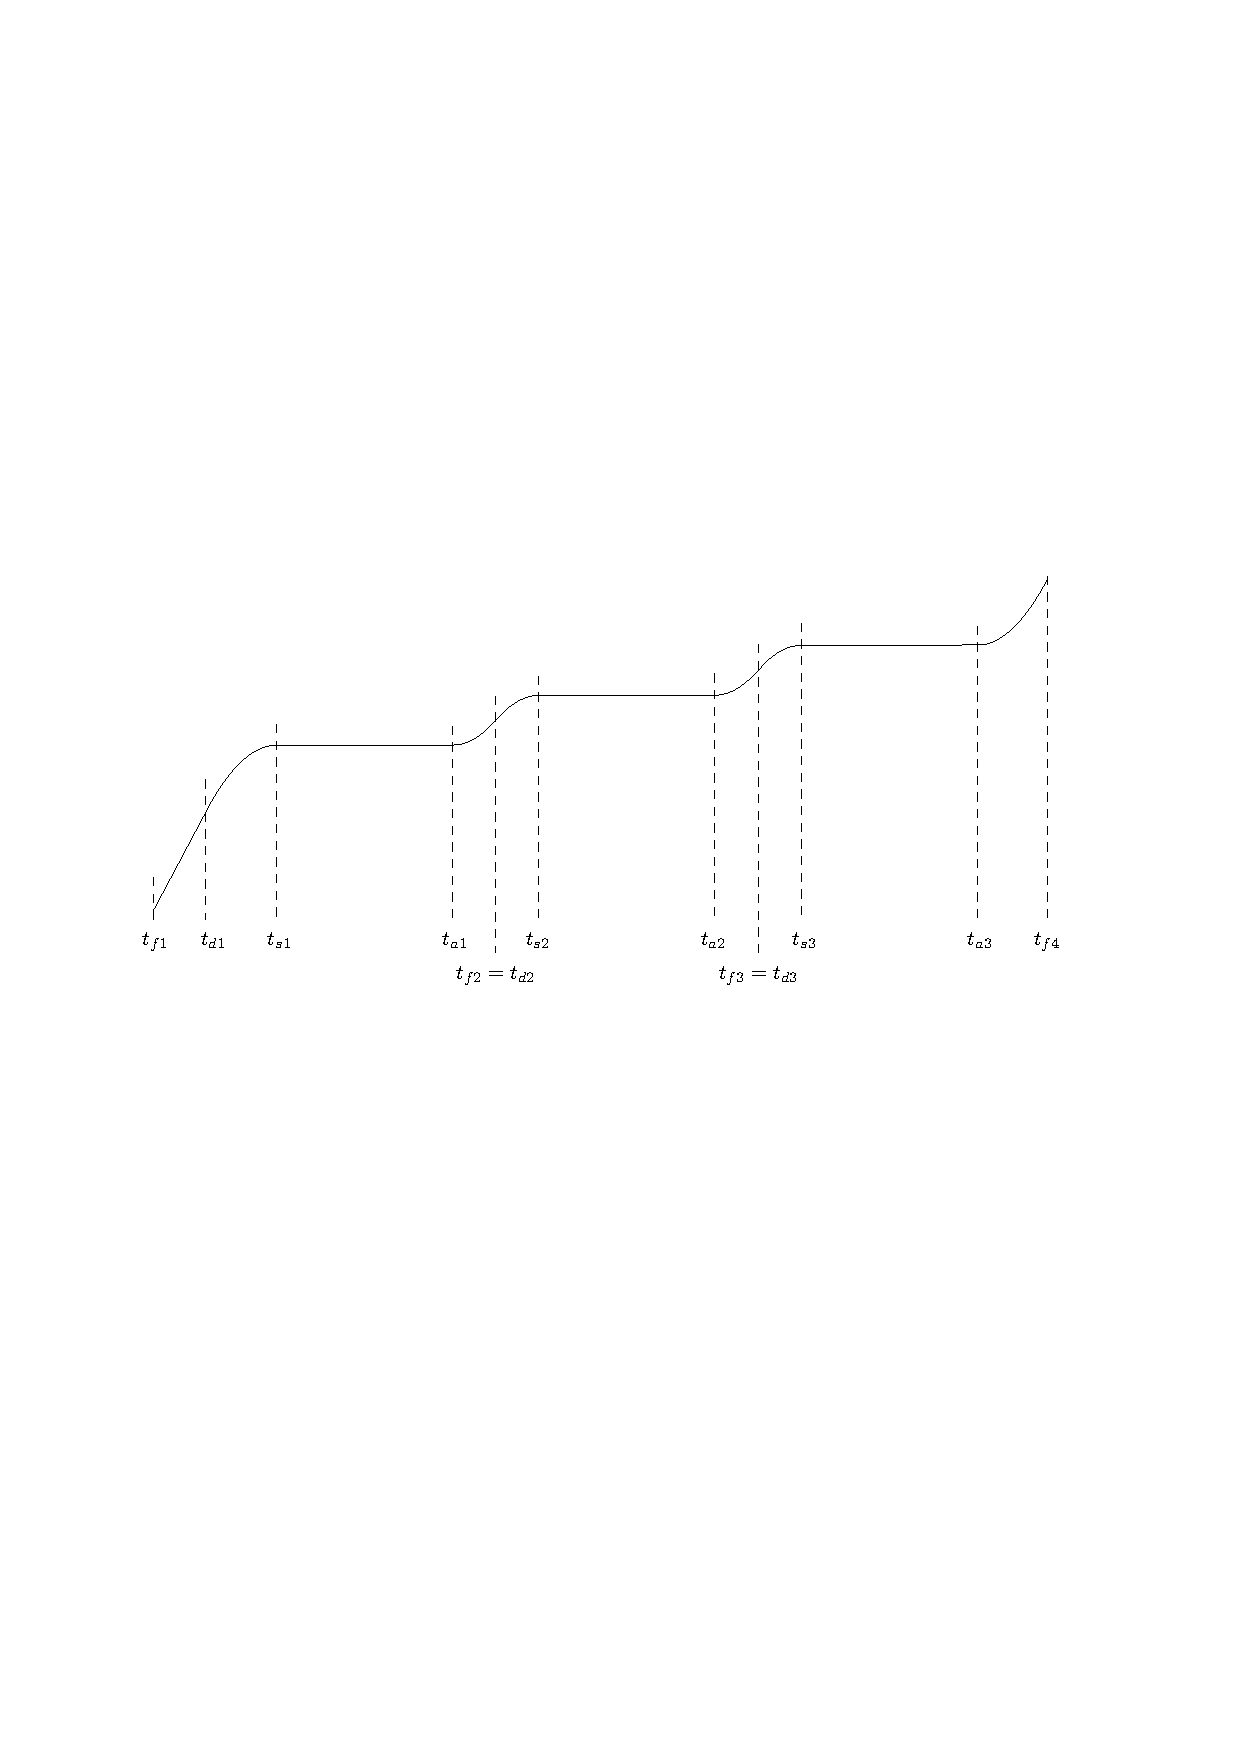
\includegraphics[scale=0.9]{figures/motion/tandem_trajectory}
  \caption{Some example of an alternating vehicle trajectory. The particular
    shape of this trajectory is due to two preceding vehicles, which causes the
    two \emph{bumps} at the times where these vehicles depart from the lane.}
  \label{fig:tandem_trajectory}
\end{figure}

Observe that an alternating trajectory $\gamma \in \mathcal{D}[a,b]$ can be described
as a sequence of four types of consecutive repeating phases, see
Figure~\ref{fig:tandem_trajectory} for an example.
%
In general, there exists a partition of $[a,b]$, denoted by
\begin{align*}
  a = t_{f1} \leq t_{d1} \leq t_{s1} \leq t_{a1} \leq t_{f2} \leq t_{d2} \leq t_{s2} \leq t_{a2} \leq \dots \leq t_{f,n+1} = b,
\end{align*}
such that we have the consecutive intervals
\begin{alignat*}{3}
  F_{i} &:= [t_{f,i}, t_{d,i}] \quad &\text{ (full speed), } \quad
  S_{i} &:= [t_{s,i}, t_{a,i}] \quad &\text{ (stopped), } \\
  D_{i} &:= [t_{d,i}, t_{s,i}] \quad &\text{ (deceleration), } \quad
  A_{i} &:= [t_{a,i}, t_{f,i+1}] \quad  &\text{ (acceleration), }
\end{alignat*}
%
such that on these intervals, $\gamma$ satisfies
%
\begin{alignat*}{3}
  &\dot{\gamma}(t) = 1 && \text{ for } t \in F_{i} , \quad \quad
  &&\dot{\gamma}(t) = 0 && \text{ for } t \in S_{i} ,\\
  &\ddot{\gamma}(t) = -\omega \quad && \text{ for } t \in D_{i} , \quad \quad
  &&\ddot{\gamma}(t) = \bar{\omega} \quad && \text{ for } t \in A_{i} .
\end{alignat*}
%
We will define parameterized functions $x^{1}$, $x^{-}$, $x^{0}$, $x^{+}$ to
describe $\gamma$ on each of these four types of intervals.
%
In the next section, we will show that this makes the smoothing procedure
particularly simple.

\subsection{Calculating smoothing times}

{\color{Navy}Derive $x^{+}$ similarly to how we derived $x^{-}$ when we
  introduced the deceleration boundary.}

It can be shown that smoothing introduces a part of deceleration $x^{-}$ only
between the four pairs of partial trajectories
\begin{align*}
    x^{+} \rightarrow x^{+} , \quad \quad
    x^{+} \rightarrow x^{0} , \quad \quad
    x^{1} \rightarrow x^{+} , \quad \quad
    x^{1} \rightarrow x^{0} .
\end{align*}
%

\section{Feasibility as system of linear inequalities}

{\color{Navy} Show that the follow constraint $a_{i} \geq \bar{a}_{i}$ can be written in terms of $a_{i-1}$.}

We need to express the entry space constraint, condition (iv) in
Lemma~\ref{lemma:necessary-conditions}, in terms of the schedule times. Recall
that this conditions requires that
\begin{align}
  \bar{x}_{i} \geq \check{x}_{i} .
\end{align}
We will show that this condition can be rewritten in the form
\begin{align}
  a_{i} \geq \check{a}_{i}(a) ,
\end{align}
where $\check{a}_{i}(a,b)$ denotes some expression of the schedule times
$a_{1}, \dots, a_{n}$.

In conclusion, feasibility is expressed through the system of linear
inequalities
\begin{subequations}
\begin{align}
  b_{i} - a_{i} &\geq B - A &\text{ for all } i \in \{1, \dots, N\}, \\
  a_{i} &\geq  a_{i-1} - 1/\omega &\text{ for all } i \in \{2, \dots, N\} , \\
  b_{i} &\geq  b_{i-1} - 1/\omega &\text{ for all } i \in \{2, \dots, N\} , \\
  a_{i} &\leq \check{a}_{i}(a) &\text{ for all } i \in \{2, \dots, N \} .
\end{align}
\end{subequations}

\begin{figure}
  \centering
  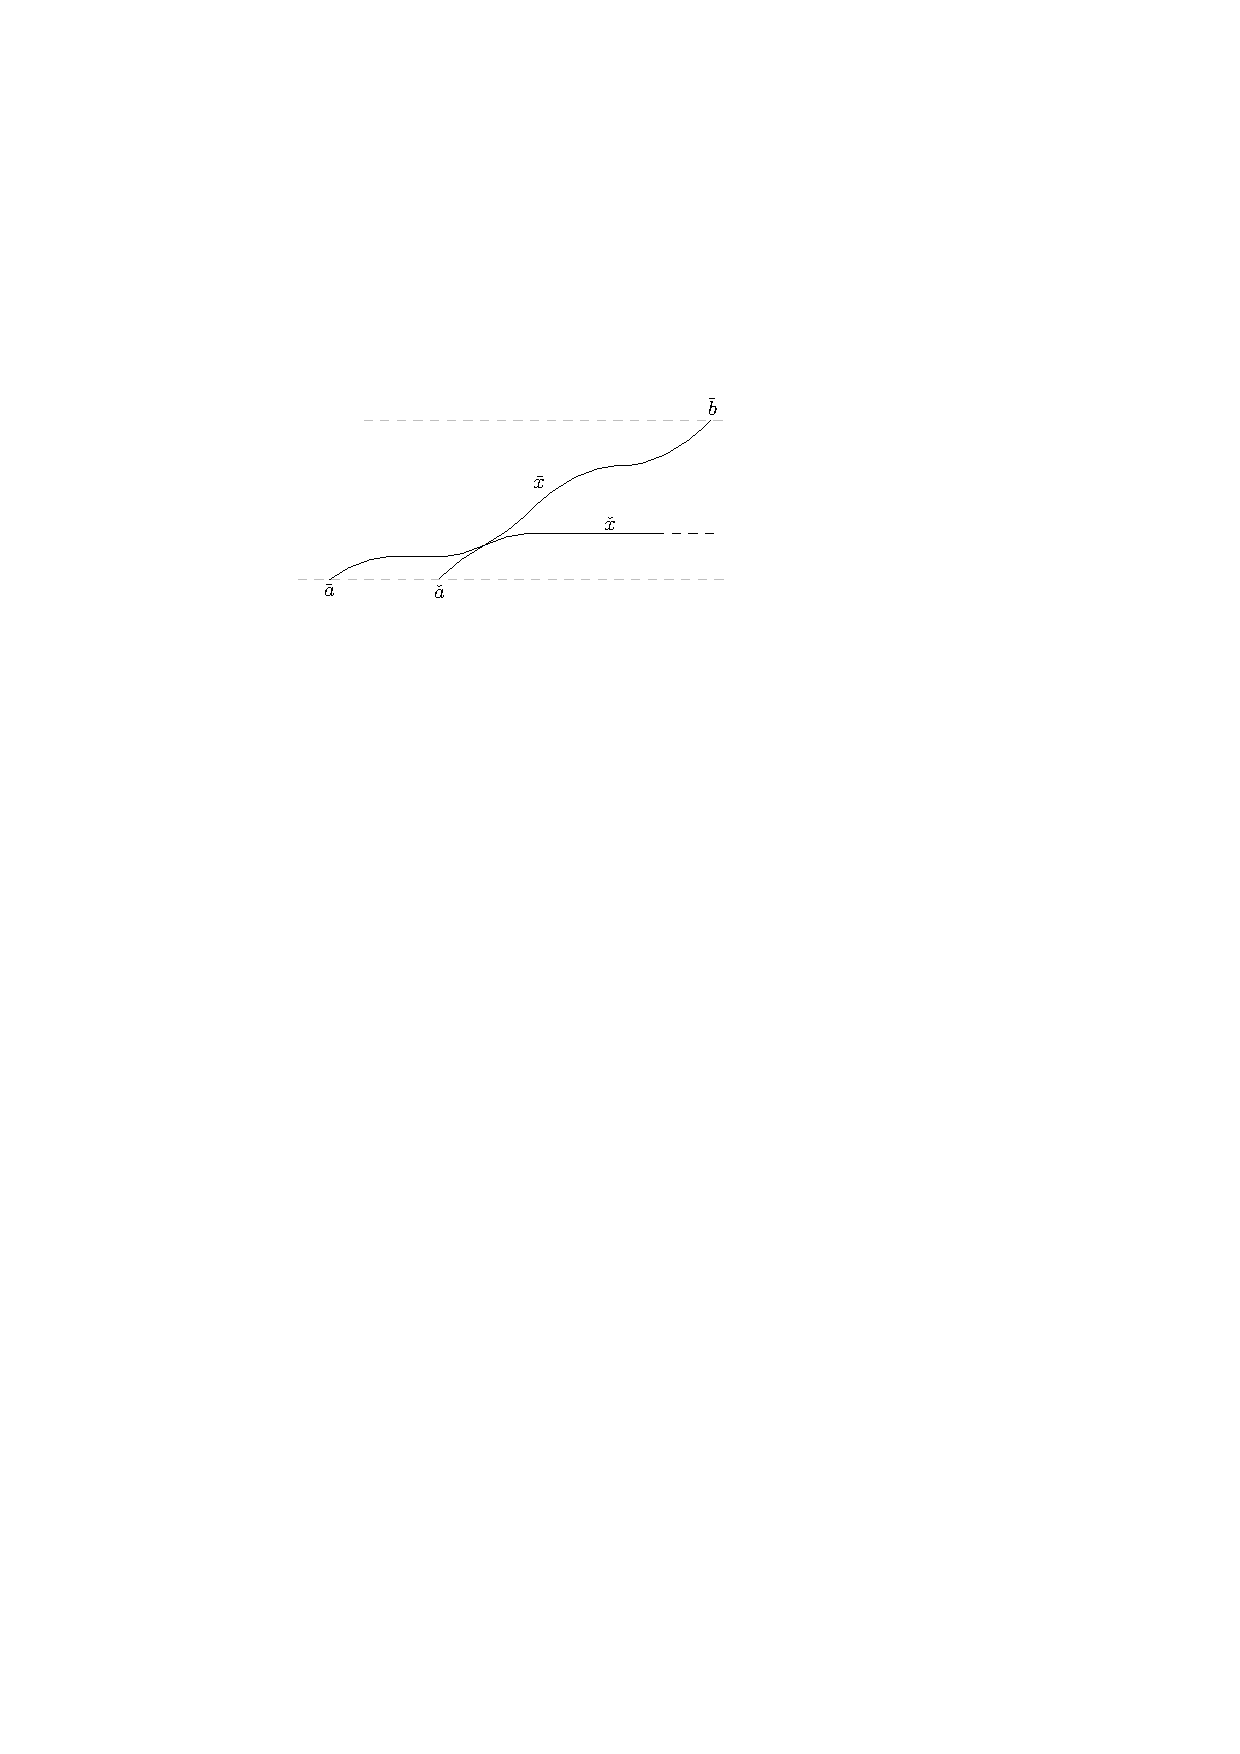
\includegraphics[scale=1]{figures/motion/rough/bufferconstraint}
  \caption{Illustration of entry space constraint and the induced minimum entry
    time $\check{a}$.}%
  \label{fig:bufferconstraint}
\end{figure}

\begin{figure}
  \centering
  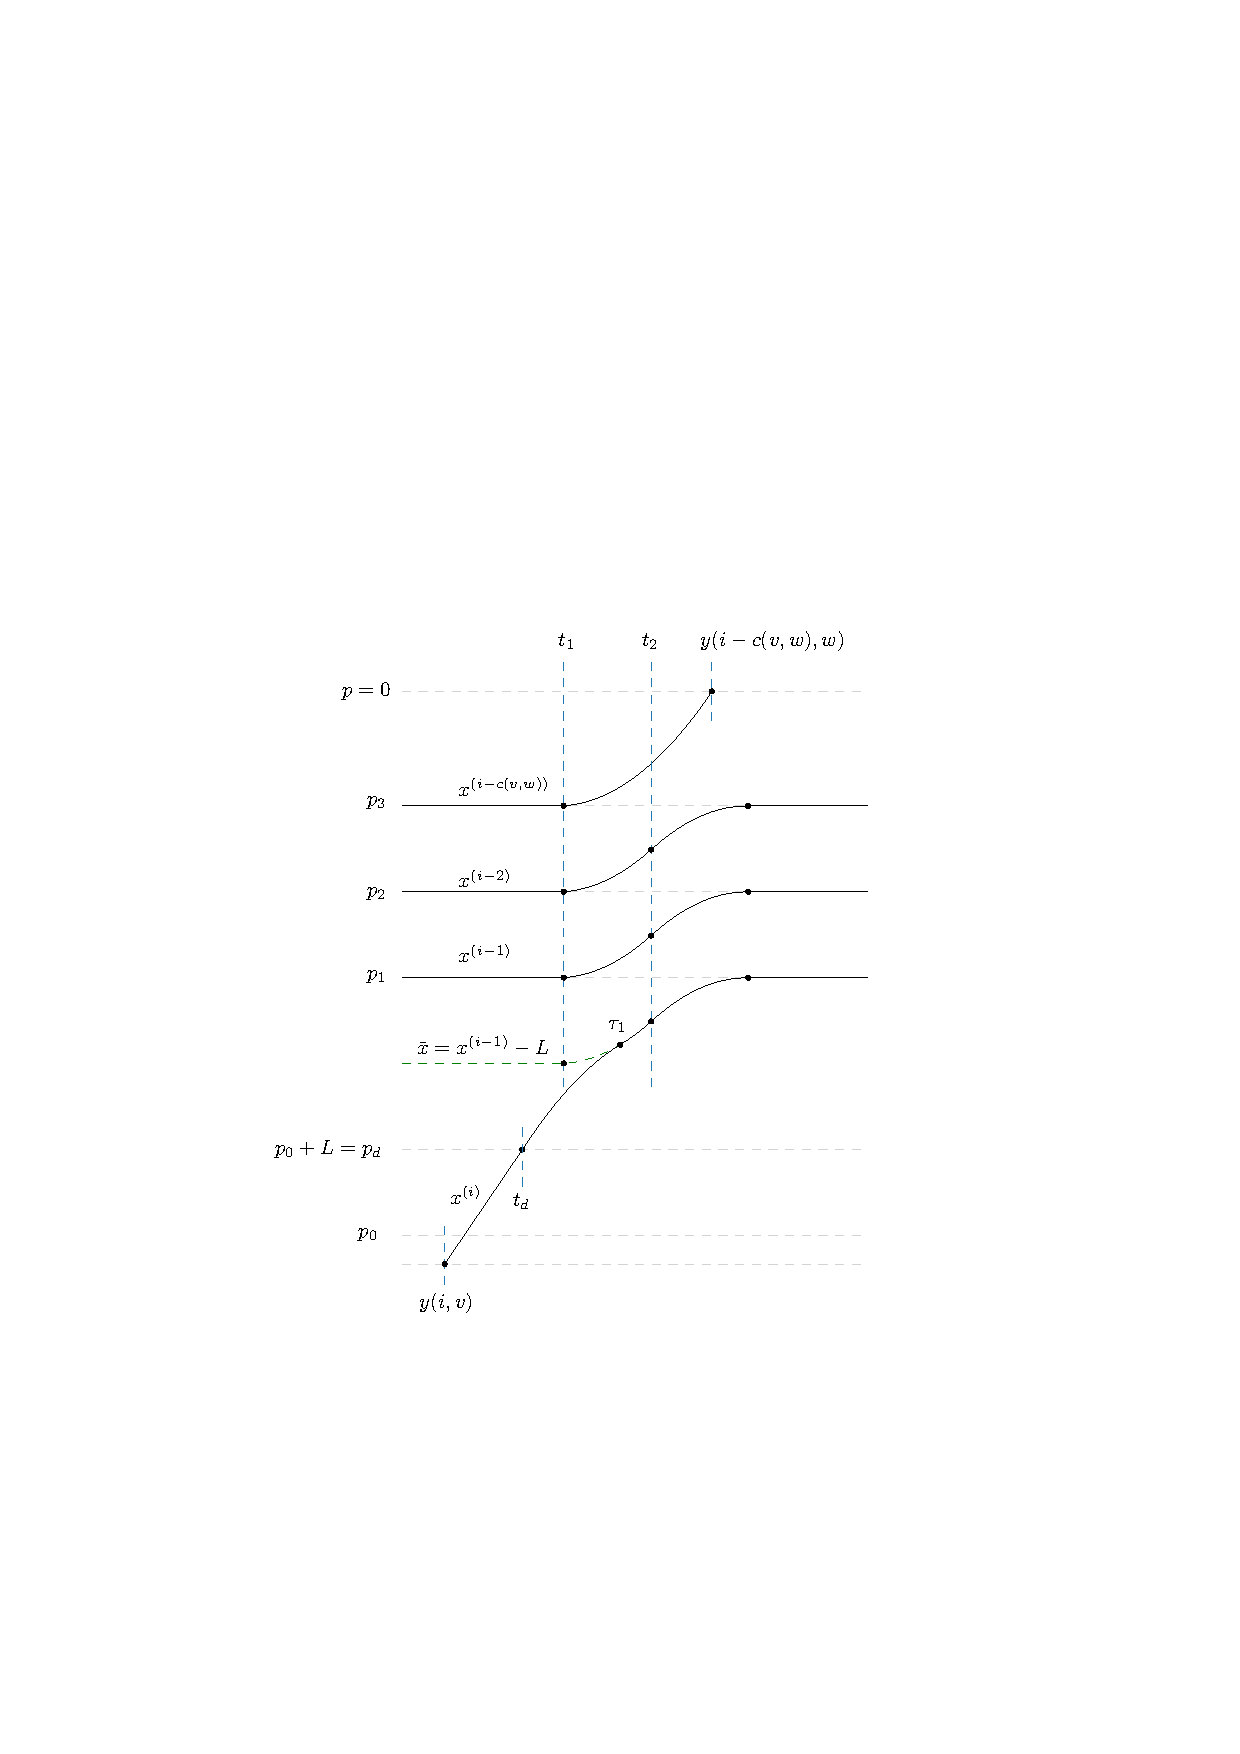
\includegraphics[scale=1]{figures/motion/example1}
  \caption{{\color{Navy} We include this old sketch here temporarily, which is
      related to derive entry space constraint in terms of schedule times.}}%
\end{figure}


\newpage
\appendix
\section{Miscellaneous}

\begin{lemma}\label{lemma:levelset}
  Let $f :\mathbb{R}^{n} \rightarrow \mathbb{R}^{m}$ be continuous and
  $y \in \mathbb{R}^{m}$, then the level set $N := f^{-1}(\{ y \})$ is a closed
  subset of $\mathbb{R}^{n}$.
\end{lemma}
\begin{proof}
  For any $y' \neq y$, there exists an open neighborhood $M(y')$ such that
  $y \notin M(y')$. The preimage $f^{-1}(M(y'))$ is open by continuity.
  Therefore, the complement
  $N^{c} = \{ x : f(x) \neq y \} = \cup_{y' \neq y} f^{-1}(\{y'\}) = \cup_{y' \neq y} f^{-1}(M(y'))$
  is open.
\end{proof}

\begin{lemma}\label{lemma:inf-continuous}
  Let $f : X \times Y \rightarrow \mathbb{R}$ be some continuous function. If
  $Y$ is compact, then the function $g : X \rightarrow \mathbb{R}$, defined as
  $g(x) = \inf \{ f(x,y) : y\in Y\}$, is also continuous.
\end{lemma}

\end{document}

% to enable the minted package
% Local Variables:
% TeX-command-extra-options: "-shell-escape"
% End:
